\chapter{Introduction}
\label{sec:introduction}

This work investigates the implementation of Latent Semantic Analysis (LSA) for discovering the main concepts in texts, in order to present a content overview of a text, or a collection of texts in the form of a tag cloud.\\
\\
1. introductory words, why is this work being written \\
2. mention information retrieval, lsa, tag clouds - generally\\
3. mention cms ? document collections ? content ? \\
4. mention the work of david mugo \\
\\
During the last decade there have been constant optimizations in information retrieval effectiveness, making web search the preferred source of finding information. A substantial part of information retrieval deals with providing access to unstructured information in various domains. Information retrieval (IR) refers to finding material (usually documents) of an unstructured nature (usually text) that satisfies an information need from within large collections (usually stored on computers) \cite{Mann08}. Many people today use methods from the field of IR when they use a search engine online, or search through their emails. In this context "unstructured data" refers to data which does not have a clear structure. As an example, unstructured data is the opposite of the structured data stored in a relational database.    \\

Information retrieval systems vary by the scale at which they operate. Three main types of IR systems can be distinguished - for web search, for personal IR, and systems performing domain-specific search. In web search IR systems, IR is done over billions of documents, stored on millions of distributed computers. Personal IR is performed at the level of consumer operating systems. And in the case of domain-specific or enterprise search, IR tasks are executed on collections of documents stored on centralized file systems, while search over the collection is provided by a handful of dedicated server machines. \\

IR technologies find wide application - in search engines, for browsing or filtering document collections, for further processing a set of retrieved documents. Before retrieval the documents are indexed, otherwise at each search, they would have to be scanned through for each query. Generally said, the index maps the words or terms back to the documents where they occur. An interesting technique for document indexing and retrieval, which will be applied in this work, is called latent semantic analysis (LSA). It indexes the document collection by representing it as a reduced matrix of words and documents. LSA representation improves IR performance with respect to a basic problem of word-matching search - synonymy, or the case when more than one term describe the same concept. \\

While IR deals with retrieval of documents, other systems manage content, such as documents. Content management includes a set of technologies and processes that support the creation, management and publication of content in any form or medium. Content may be documents, multi-media files, or any other file types that follow content lifecycle and require management. Content management systems (CMS) vary depending on their purpose and target environments - there are CMS for the web, for enterprise, for mobile devices, as well as CMS for management of document collections, also called document management systems (DMS). \\

%
% DMS simplified image
%
\begin{figure}[htbp]
	\centering
	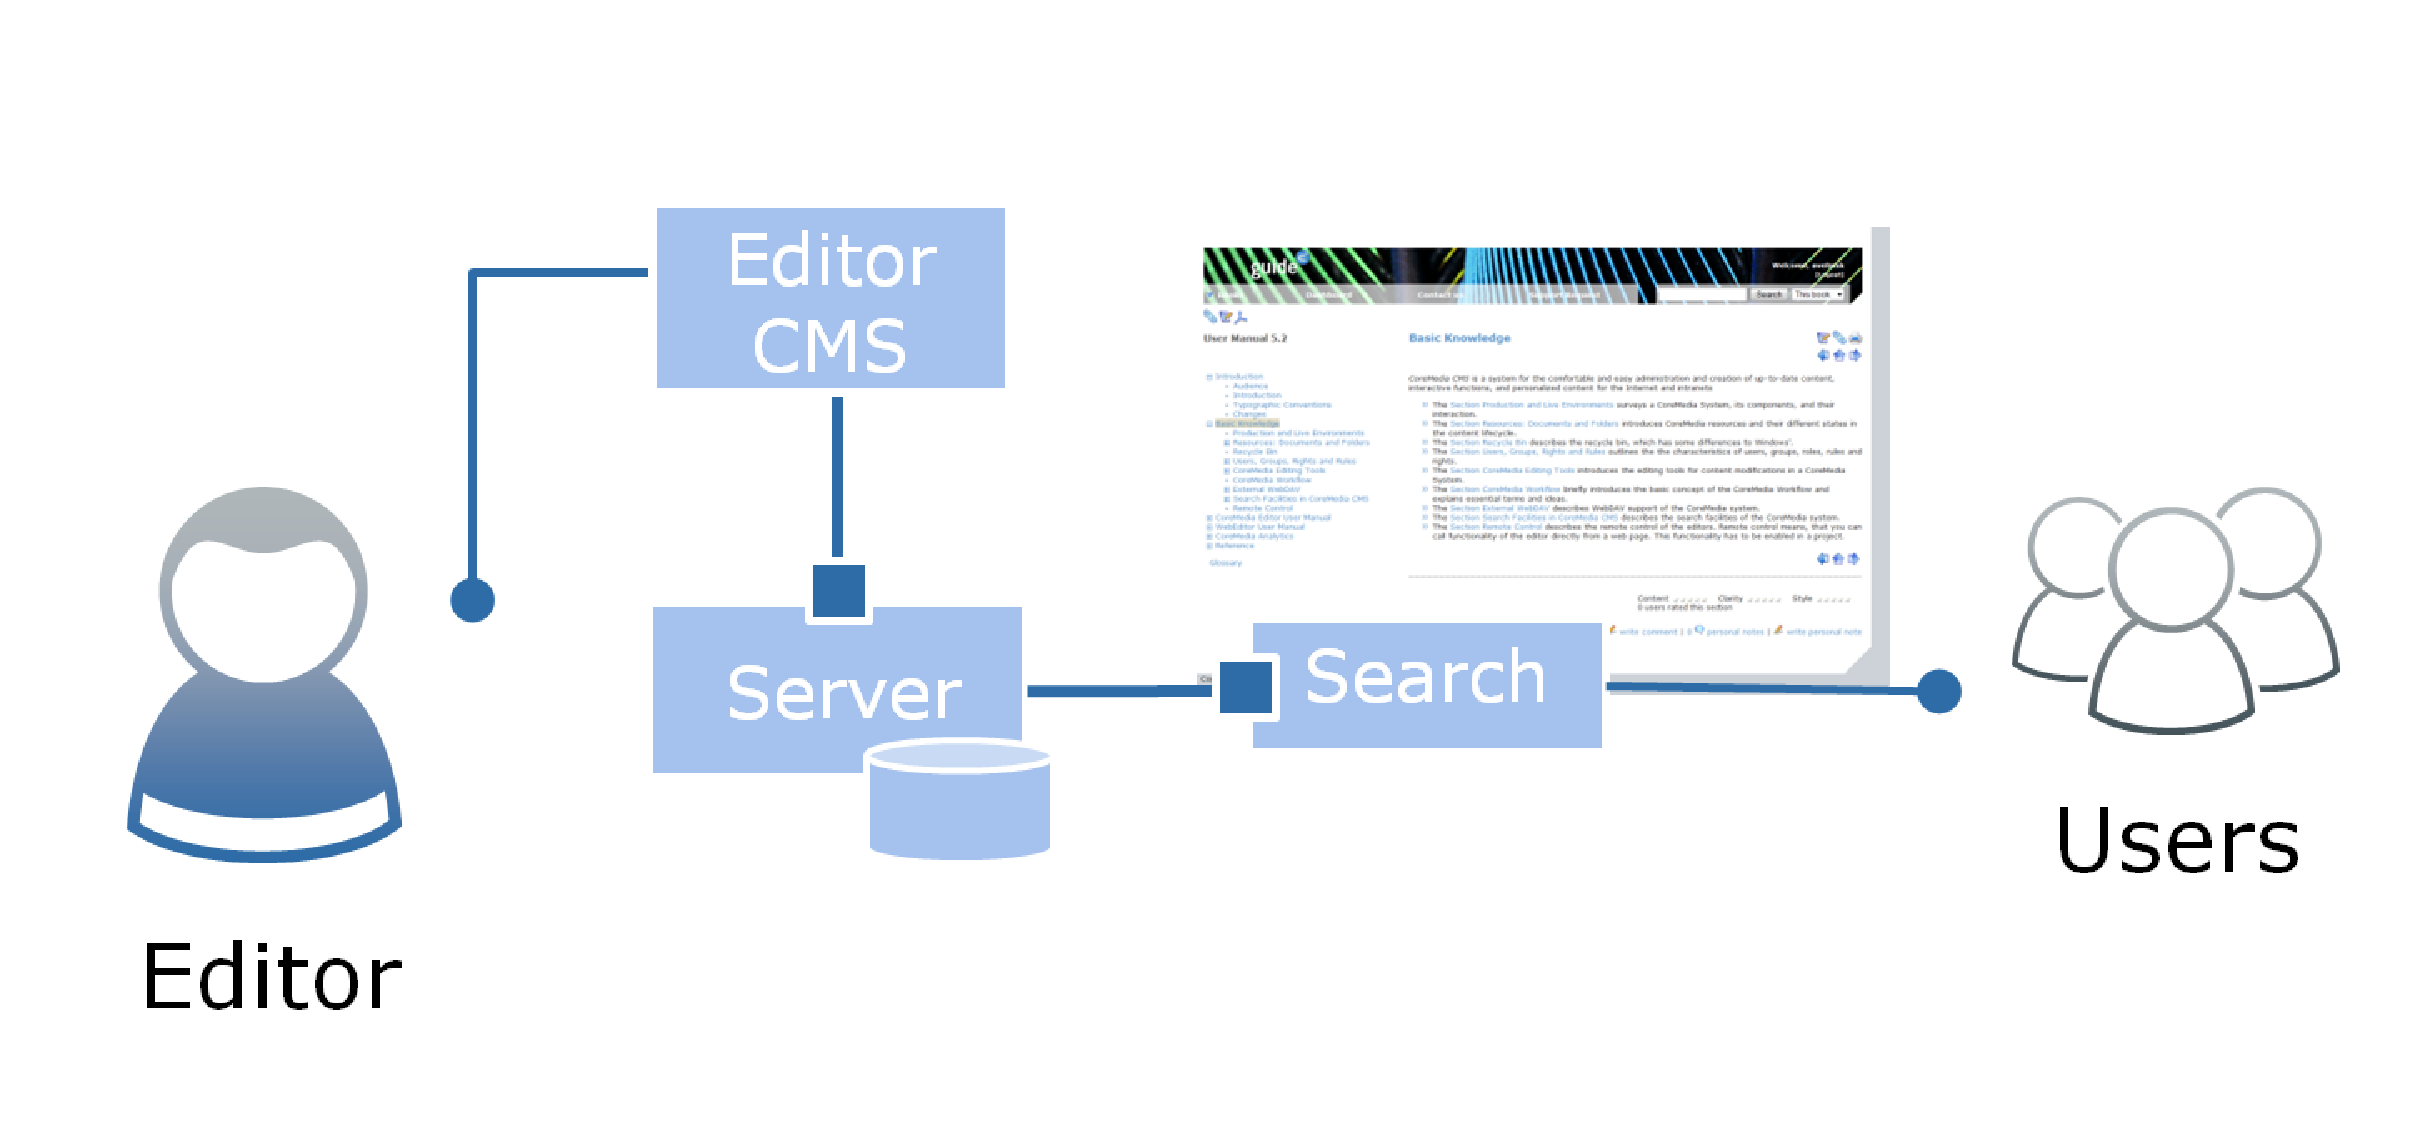
\includegraphics[width=\ScaleIfNeeded]{img/cms-simplified} 
 % or [scale=0.5]
	\caption{ Online Document Management System }
	\label{fig:docmachine}
\end{figure}

Figure~\ref{fig:docmachine} shows a simplified document management system, offering online access to its content. Using the editor CMS, editors can create, edit or delete content, which is managed and stored by a Content Management Server. Content is presented to the end users, who can access the document collection and search through it according to their information need. CMS usually consists of an environment for content management, and an environment for content delivery or presentation. However, in the introduction we only outline the basic concepts of the system. \\


\section{Motivation and objective}
\label{sec:introduction:motandobj}  
A drawback of the classical LSA implementation as an information retrieval method is the low precision of the returned results. A previous work by David Mugo \cite{mugo10} has investigated the improvement of LSA precision performance by annotating the document collection and including the anotations used in LSA. In his work, Mugo constructs a concept-document matrix from the annotations used, and concatenates it with the word-document matrix normally generated in LSA process. The proposed solution, however, results in a slow speed of LSA, and has left Mugo's hypothesis open. \\

Taking into consideration the results from Mugo's work, the current project has several objectives to reach. It will investigate the implementation of LSA method for improving information retrieval in a domain-specific document management system with respect to context-based search. A further investigation will be made on improving the precision performance of LSA method by using semantic annotations, and on finding an adequate way to present the results of LSA as a tag cloud. And finally, it will be investigated how to use the tag cloud as a form of a relevance feedback to control LSA method. \\

In the context of the stated objectives, semantic annotations are meta data annotations used to add information to unstructured data, or to the document collection. Semantic annotations are based on an ontology in our case, specifically developed for the domain of interest CoreMedia CMS. Ontologies are used to capture some knowledge about a certain domain, by describing the concepts of the domain and the relationships between them. To further clarify the objectives, relevance feedback is an IR technique, used to influence the retrieved results based on the user's preference. It allows the user to modify the initial tag cloud by selecting the most relevant words. The tag cloud is then re-generated from LSA results with the relevance feedback posted as a query. \\

\section{Outline}
\label{sec:introduction:outline}
The reminder of this work is organized as follows. Chapter \ref{sec:docmanagsystem} describes in more detail what a document management system is, and provides an overview of the general structure of DocMachine 2.0, the DMS deployed at CoreMedia AG. Chapter \ref{sec:semannot} presents the basic concepts of ontologies and document annotations based on ontologies. In Chapter \ref{sec:lsa} an overview of latent semantic analysis method is given, as well as an approach for improving LSA's precision by including semantic annotations in the method. Chapter \ref{sec:implementation} presents the prototype implementation and makes an evaluation of the results achieved in this work. And finally, conclusions are drawn in Chapter \ref{sec:conclusion}, along with some limitations of the current study and outlook for a future research.   \\ 
